\chapter{Funcionament d'un expenedor automàtic de begudes fredes}\label{chapter:funcionament d'un expenedor}
Per a poder dissenyar la solució i poder entendre les millores, primer s'ha d'esbrinar i entendre el funcionament original d'un expenedor automàtic.

\section{Descripció de les parts}
La descripció de les parts es pot trobar al manual d'instruccions de l'expenedor\autocite{vender-instructions} a l'Apèndix~\ref{app:vender}.

\section{Cas d'ús}
Presentem el cas d'ús usual:
\begin{enumerate}
\item Un usuari s'acosta fins l'expenedor i observa quins productes estan disponibles i quin preu tenen. Cada botó de selecció té una etiqueta al costat que indica el producte i el seu preu. La disponibilitat del producte la indica un indicador lluminós sota el botó (si emet llum, no està disponible.
\item Un cop l'usuari ha fet la seva elecció, introdueix monedes amb un valor igual o superior a l'import del producte.
\item L'usuari apreta el botó de selecció del producte que ha escollit.
\item L'expenedor retorna el canvi (si n'hi ha) i serveix la beguda que l'usuari ha seleccionat.
\end{enumerate}

Exposem els casos d'ús quan alguna cosa va com no hauria d'anar:
\begin{description}[font=\normalfont\textbf]\itemsep2pt 
\vspace{-1em}
\parskip1pt \parsep0pt
\item[L'usuari apreta el botó d'un producte que no està disponible:] No passa res. És com si no hagués apretat cap botó.
\item[L'usuari apreta el botó d'un producte pel qual no té saldo suficient:] No passa res. És com si no hagués apretat cap botó.
\item[L'indicador de "import exacte" està encès:] L'expenedor només accepta monedes del tipus que pot retornar i no retorna canvi.
\vspace{-1em}
\end{description}

\section{Circuit elèctric}
L'expenedor automàtic està dissenyat per funcionar amb un sistema electromecànic sense necessitat de circuits electrònics.

El mecanisme consistia en un petit interruptor mecànic amb una palanqueta allargada que quedava premuda quan s'introduïa un tipus de moneda concret i activava la resta del circuit que era controlat per un relé de tres commutadors, els botons de selecció i els interruptors que es troben on els carrils per controlar la posició dels motors.

Avui dia, amb expenedors que retornen el canvi, aquest relé és substituït per la màquina de canvi, que és l'aparell que classifica les monedes segons el seu valor, i després retorna canvi si cal. A més, dona la possibilitat de poder definir diversos preus.

Per tal de tenir una visió més clara del funcionament per tal de poder dissenyar el nostre sistema, presentem un circuit simplificat de l'expenedor juntament amb la màquina de canvi que s'ha extret del manual d'instruccions (llegint les explicacions i analitzant l'esquema elèctric complet).

\begin{figure}[H]
\center
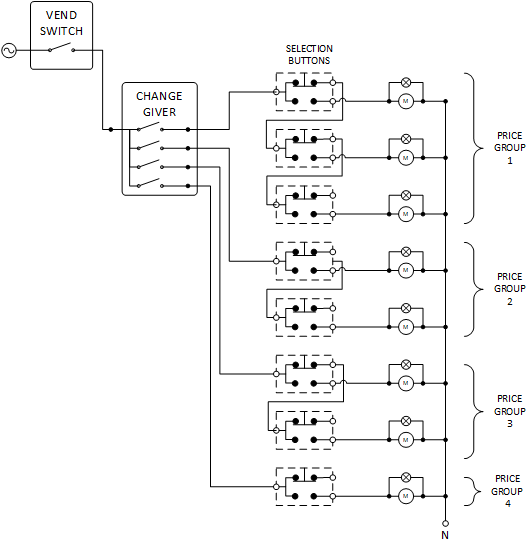
\includegraphics[width=0.8\textwidth]{images/vender_electrical}
\caption{Esquema elèctric simplificat de l'expenedor}
\label{fig:vender_electrical}
\end{figure}

Quan s'introdueixen les monedes, la màquina de canvi dona corrent als botons pels quals s'ha introduit un import suficient. Un cop premut el botó de selecció, es tanca el circuit del motor i el motor s'acciona. Hi ha mes factors a tenir en compte, però per a dissenyar el nostre sistema ja en tenim suficient.

Els botons de selecció estan connectats en serie d'aquesta manera en concret per evitar que el circuit el tanqui més d'un botó al mateix temps.

Com podem veure a l'esquema, abans de la màquina de canvi hi ha un interruptor. Aquest interruptor obre el circuit quan es deshabilita la venda en casos com quan no queda producte a cap carril de l'expenedor, o s'està servint una beguda o bé quan hi ha algun problema amb el mecanisme de l'expenedor i s'ha encallat.

Quan es deshabilita la venda, la màquina de canvi ja no accepta més monedes però l'import de les monedes que s'hagi introduït abans no es perd. Quan es torna a habilitar la venda es pot seguir comprant amb el saldo anterior. Si s'apreta la palanca de retorn  mentre la venda està deshabilitada la màquina de canvi retorna els diners introduïts.

Malauradament, si l'expenedor es queda sense energia durant el procés de compra, es perd l'import introduït.

Les làmpades que hi ha en paral·lel amb els motors tenen dues funcions:
\begin{enumerate}
\item Si estan enceses durant el període entre que s'ha apretat el botó de selecció i s'ha servit la beguda, indica que el circuit s'ha tancat correctament i que el motor d'aquell carril està girant.
\item Si estan enceses durant de forma permanent indiquen que ja no queda producte en aquell carril.
\end{enumerate}